\section{Combining MRST and Gmsh}
\label{sec:combining}
As MRST and Gmsh both have their limitations, adopting Gmsh into an MRST workflow may be beneficial. This section will discuss an existing method for loading Gmsh meshes, \nameref{sec:GmshToMRST}, and introduce a new package for integrating the two, \nameref{sec:own_software}.

\subsection{\texttt{gmshToMrst}}
\label{sec:GmshToMRST}
Originally developed by \textcite{gmsh_to_mrst} as a stand-alone method for loading Gmsh meshes into MRST, \verb|gmshToMrst| became part of MRST's module library with release \verb|2022a|. The module reads the mesh from an \verb|.m|-file and performs the necessary computations for converting the mesh to an MRST grid. While it does this job well, one key requirement of \verb|gmshToMrst| is that the Gmsh mesh has been computed beforehand. This requires users to manually create the Gmsh mesh, slowing down the rapid prototyping MRST is designed to perform, while forcing its users to learn an entirely new program in order to generate the grids.

% \verb|gmshToMRST| is a MATLAB module for loading created Gmsh meshes. 

\subsection{\texttt{gmsh4mrst}}
\label{sec:own_software}
To help with this, I have developed a new software module, \verb|gmsh4mrst|, to enable automatic Gmsh mesh generation from MATLAB. By abstracting most of the manual work required for generating meshes in Gmsh, \verb|gmsh4mrst| is designed to enable users to use Gmsh as a backend for mesh creation, speeding up the mesh generation of detailed domains, without the user having to spend time learning a new software. The goal of \verb|gmsh4mrst| is to enable a near drop-in replacement of \verb|distmesh| with Gmsh-created meshes.


\subsubsection{Installation of \texttt{gmsh4mrst}}
In order to integrate the two systems, \verb|gmsh4mrst| is split in two parts, one written in Python and one in MATLAB. The Python package is hosted on PyPi \cite{gmsh4mrst}, and can easily be installed from there. The MATLAB package must be manually downloaded, and the files must be added to the MATLAB path.

The Python package works as a stand-alone package. The MATLAB package, however, uses Python to create base meshes, and therefore requires that the Python package is installed to run. MATLAB must be run from an environment with the Python package installed, whether that is through a virtual environment or the base Python installation on the computer.


\subsubsection{Features of \texttt{gmsh4mrst}}
The primary target of \verb|gmsh4mrst| is to automate Gmsh mesh creation for use in MRST grids, while maintaining the flexibility needed for optimal grid creation. Care has been taken to ensure \verb|gmsh4mrst| is as robust as possible, especially when it comes to connecting MATLAB and Python.

One key feature of \verb|gmsh4mrst| is its many user-settable arguments and parameters. By leaving most grid-refinement decisions available to the user, \verb|gmsh4mrst| can be used for almost every grid creation necessary, while reasonable defaults ensure the module can be used for simple grids without much time spent on refinement. An overview of the available arguments is given in Appendix~\ref{app:gmsh4mrst-arguments}.

The module easily handles complex, non-convex domains, and the goal of the module is to precisely and quickly adapt the grid to all given face- and cell constraints. An example of the output from the module can be seen in \autoref{fig:gmsh4mrst-pymethods} and \autoref{fig:gmsh4mrst-MATLABmethods}.

\subsubsection{Using \texttt{gmsh4mrst} in Python}
The Python part of \verb|gmsh4mrst| is where most of the grid generation is done. While the actual implementation and specifications may change over time, the Python package currently implements three methods.

\paragraph{\texttt{background\_grid\_2D}:}
The most basic of the implemented methods, \verb|background_grid_2D| uses Gmsh to create a simple background triangulation without any embedded points or lines, but with refinement around face- and cell constraints. This results in a uniform mesh, and can be used as a straight replacement of the Distmesh algorithm. The user has detailed control of the mesh, including any refinement done along the constraints.

\paragraph{\texttt{delaunay\_grid\_2D}:}
Going one step further, \verb|delaunay_grid_2D| creates a background triangulation, but include the constraints in the generated mesh. Face constraints are embedded directly as lines or points, ensuring that the faces of the resulting Delaunay triangulation align with the constraints. Each cell constraint is wrapped in a transfinite mesh, ensuring the constraints are traced with cells in the triangulation. As a result of using transfinite meshes, \verb|delaunay_grid_2D| fails if any cell constraints intersect either each other or any face constraints.

\paragraph{\texttt{pebi\_base\_2D}:}
The most complex of the implemented methods, \verb|pebi_base_2D| creates a background triangulation, but include both face- and cell constraints as transfinite meshes. The idea behind this is that it ensures a distribution of Delaunay vertices -- and by extension PEBI sites after converting the triangulation -- around the constraints, ensuring face constraints are traced by PEBI faces and cell constraints by PEBI sites. As a result of using transfinite meshes, \verb|pebi_base_2D| fails if any constraints intersect.

All methods implemented in the Python package output Delaunay triangulations. The difference in outputs of the methods is shown in \autoref{fig:gmsh4mrst-pymethods}, where the left sides of the grids contain face constraints, and the right sides contain cell constraints.

\begin{figure}[p]
    \centering
    \begin{subfigure}[b]{0.49\textwidth}
        \centering
        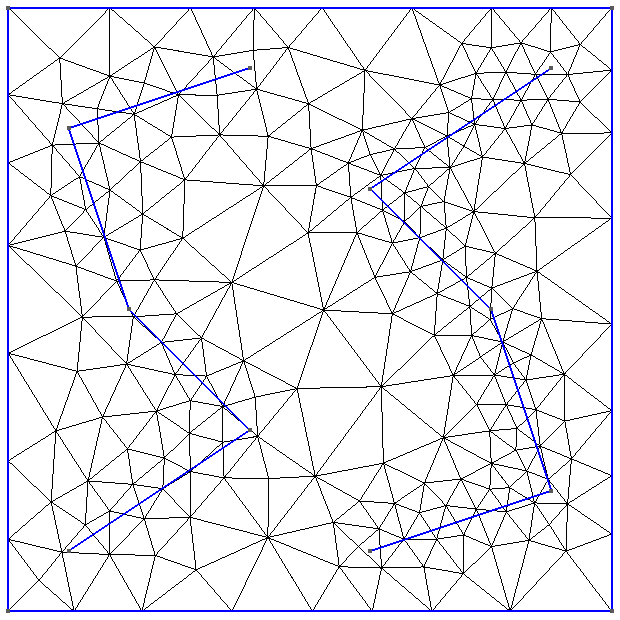
\includegraphics[width=\textwidth]{report/Images/Combining software/Demo gmsh4mrst/demo_background_grid_2D_lines.png}
        \caption{\texttt{background\_grid\_2D}}
        \label{fig:background_grid_2D}
    \end{subfigure}
    \begin{subfigure}[b]{0.49\textwidth}
        \centering
        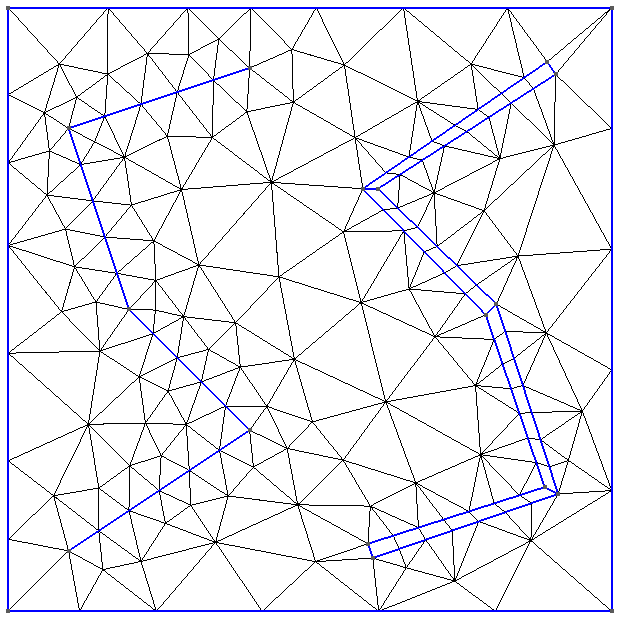
\includegraphics[width=\textwidth]{report/Images/Combining software/Demo gmsh4mrst/demo_delaunay_grid_2D_lines.png}
        \caption{\texttt{delaunay\_grid\_2D}}
        \label{fig:delaunay_grid_2D}
    \end{subfigure}
    \begin{subfigure}[b]{0.49\textwidth}
        \centering
        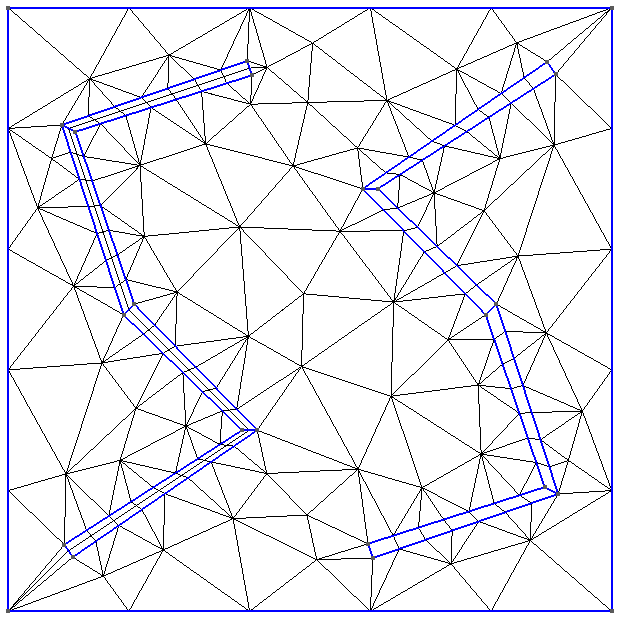
\includegraphics[width=\textwidth]{report/Images/Combining software/Demo gmsh4mrst/demo_pebi_base_2D_lines.png}
        \caption{\texttt{pebi\_base\_2D}}
        \label{fig:pebi_base_2D}
    \end{subfigure}
    \caption[Comparison of the Python methods implemented in \texttt{gmsh4mrst}]{Comparison of the Python methods implemented in \texttt{gmsh4mrst}. The grids have a fault on the left side, and a well on the right side.}
    \label{fig:gmsh4mrst-pymethods}
\end{figure}

\subsubsection{Using \texttt{gmsh4mrst} in MATLAB}
The MATLAB part of \verb|gmsh4mrst| contains all code for converting the Gmsh meshes to MRST grids, as well as some code for creating PEBI sites. While the actual implementation and specifications may change over time, the MATLAB package currently implements three methods. 

\paragraph{\texttt{pebiGrid2DGmsh}:}
Designed to be a semi-direct replacement of MRST's \verb|pebiGrid2D|, \verb|pebiGrid2DGmsh| uses \verb|background_grid_2D| to create a background grid, then creates well and fracture sites in MATLAB. This gives it the same flexibility and robustness as \verb|pebiGrid2D|, while avoiding the slow site distribution of Distmesh. The method works nicely for face constraints, but struggles somewhat with aligning cell constraints accurately.

\paragraph{\texttt{delaunayGrid2DGmsh}:}
The most direct of the MATLAB methods, \verb|delaunayGrid2DGmsh| uses \verb|delaunay_grid_2D| to create a Delaunay triangulation capturing the supplied constraints, then converts it to an MRST grid directly. As no conversion is done, this leaves the output grid as a Delaunay triangulation, but it avoids the extra work of converting without losing constraint information. Due to using \verb|delaunay_grid_2D|, no cell constraints may intersect.

\paragraph{\texttt{pebiGrid2DGmshBase}:}
A somewhat experimental method, \verb|pebiGrid2DGmshBase| uses \verb|pebi_base_2D| to create a triangulation with constraints embedded as transfinite meshes. The user can then choose whether to convert the triangulation to a PEBI grid or not. This results in a relatively flexible method, but due to using \verb|pebi_base_2D|, no constraints may intersect.

All the MATLAB methods gives the user complete control of all parameters of the underlying Python grid creation, with \verb|pebiGrid2DGmsh| additionally letting the user control the fault- and well site creation done in MATLAB. The difference in outputs of the methods is shown in \autoref{fig:gmsh4mrst-MATLABmethods}, where the left sides of the grids contain face constraints, and the right sides contain cell constraints.

\begin{figure}[p]
    \centering
    \begin{subfigure}[b]{0.49\textwidth}
        \centering
        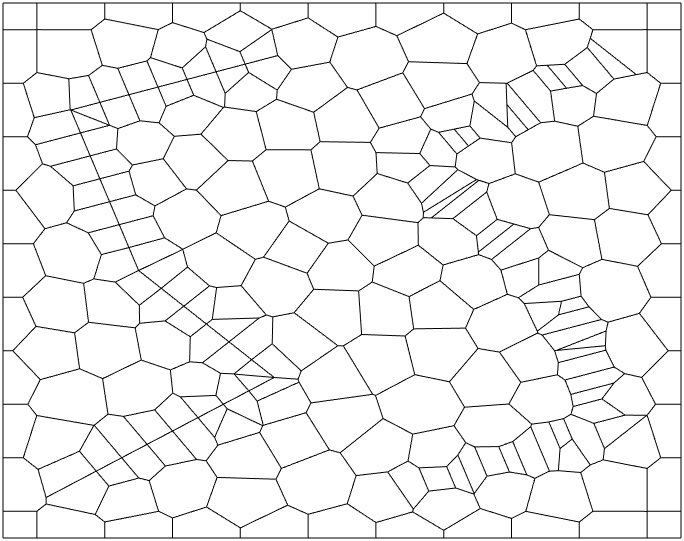
\includegraphics[width=\textwidth]{report/Images/Combining software/Demo gmsh4mrst MATLAB/demo_pebiGrid2DGmsh.png}
        \caption{\texttt{pebiGrid2DGmsh}}
        \label{fig:pebiGrid2DGmsh}
    \end{subfigure}
    \begin{subfigure}[b]{0.49\textwidth}
        \centering
        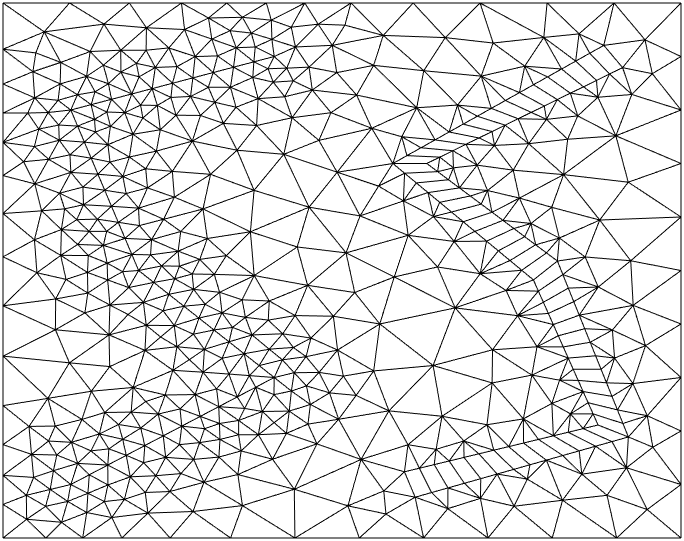
\includegraphics[width=\textwidth]{report/Images/Combining software/Demo gmsh4mrst MATLAB/demo_delaunayGrid2DGmsh.png}
        \caption{\texttt{delaunayGrid2DGmsh}}
        \label{fig:delaunayGrid2DGmsh}
    \end{subfigure}
    \begin{subfigure}[b]{0.49\textwidth}
        \centering
        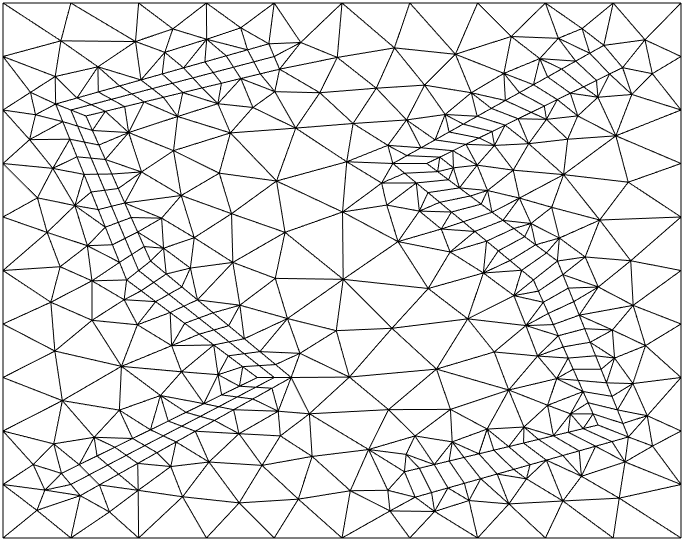
\includegraphics[width=\textwidth]{report/Images/Combining software/Demo gmsh4mrst MATLAB/demo_pebiGrid2DGmshBase.png}
        \caption{\texttt{pebiGrid2DGmshBase}}
        \label{fig:pebiGrid2DGmshBase}
    \end{subfigure}
    \begin{subfigure}[b]{0.49\textwidth}
        \centering
        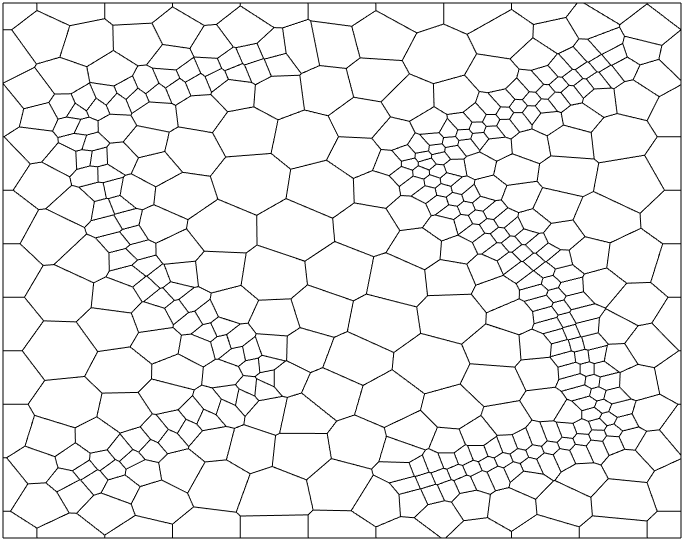
\includegraphics[width=\textwidth]{report/Images/Combining software/Demo gmsh4mrst MATLAB/demo_pebiGrid2DGmshBase_PEBI.png}
        \caption{\texttt{pebiGrid2DGmshBase} as PEBI}
        \label{fig:pebiGrid2DGmshBase_PEBI}
    \end{subfigure}
    \caption[Comparison of the MATLAB methods implemented in \texttt{gmsh4mrst}]{Comparison of the MATLAB methods implemented in \texttt{gmsh4mrst}. The grids have a fault on the left side, and a well on the right side.}
    \label{fig:gmsh4mrst-MATLABmethods}
\end{figure}


\subsubsection{Mechanics of \texttt{gmsh4mrst}}
% Deep-dive into the mechanics of gmsh4MRST
% How the different features are implemented, concretely
% Discuss Fields, constraint implementation (especially cell constraints), etc.
\paragraph{Faults as embedded lines:}
Faults are implemented differently in the three available methods, but here we discuss faults implemented as embedded face constraint lines in Gmsh, which is how it is done in \verb|delaunayGrid2D|. In Gmsh, embedding a line is a relatively simple process, but extra care is taken to ensure intersections between faults are modelled correctly. If two constraint segments intersect, both segments are split at the segment, creating four sub-segments -- two starting at the intersection and two ending at the intersection. This process is similar to the one shown in 

\paragraph{Faults as transfinite grids:}
In \verb|pebiGrid2DGmshBase|, faults are implemented as transfinite grids. By creating a structured grid around the fault, we can manually control the site distribution around the line, ensuring it ends up as a face in the final grid. We can create protective sites around the faults by increasing the number of perpendicular nodes used in the transfinite grid. When the grid is converted to PEBI, each fault grid should have an even number of perpendicular nodes to make it a face in the grid, while they should have an odd number of nodes to stay as a face in the Delaunay triangulation. An illustration of this process is shown in \autoref{fig:trans-faults}.

\begin{figure}[htp]
    \centering
    \begin{subfigure}[b]{\textwidth}
        \centering
        \begin{subfigure}[b]{0.35\textwidth}
            \centering
            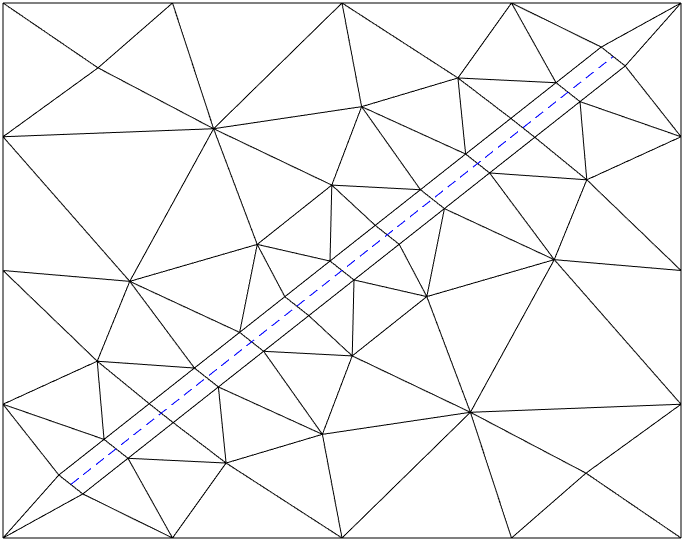
\includegraphics[width=\textwidth]{report/Images/Combining software/Faults as transfinite grids/face_constraint_as_transfinite_delaunay_1.png}
        \end{subfigure}
        \begin{subfigure}[b]{0.35\textwidth}
            \centering
            \includegraphics[width=\textwidth]{report/Images/Combining software/Faults as transfinite grids/face_constraint_as_transfinite_pebi_1.png}
        \end{subfigure}
        \caption{Fault represented by 2-width transfinite grid.}
        \label{fig:trans-fault-1}
    \end{subfigure}
    \begin{subfigure}[b]{\textwidth}
        \centering
        \begin{subfigure}[b]{0.35\textwidth}
            \centering
            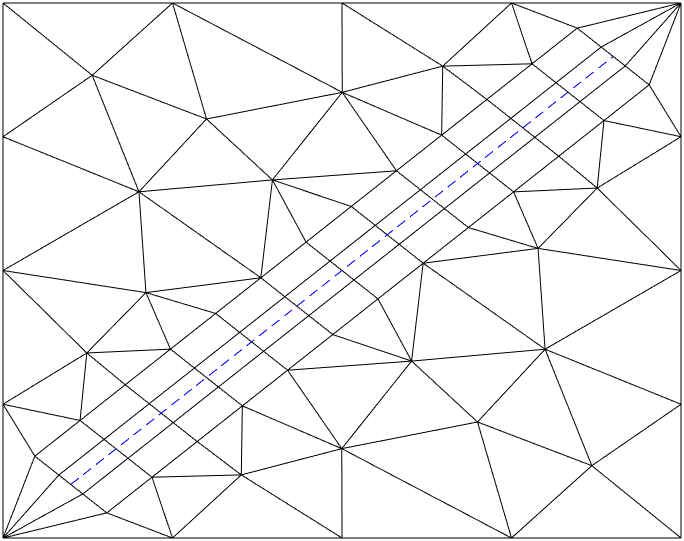
\includegraphics[width=\textwidth]{report/Images/Combining software/Faults as transfinite grids/face_constraint_as_transfinite_delaunay_2.png}
        \end{subfigure}
        \begin{subfigure}[b]{0.35\textwidth}
            \centering
            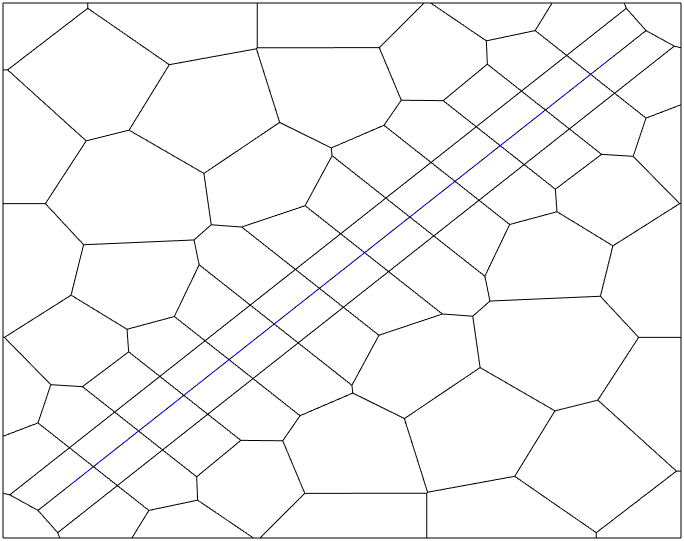
\includegraphics[width=\textwidth]{report/Images/Combining software/Faults as transfinite grids/face_constraint_as_transfinite_pebi_2.png}
        \end{subfigure}
        \caption{Fault represented by 4-width transfinite grid.}
        \label{fig:trans-fault-2}
    \end{subfigure}
    \caption[Faults represented as transfinite grids.]{Faults represented as transfinite grids. The blue line represents a fault. The plots to the left are Delaunay grids before conversion, and the plots to the right are the resulting PEBI grids after conversion.}
    \label{fig:trans-faults}
\end{figure}

\paragraph{Wells as transfinite grids:}
Wells are implemented differently in the three methods as well, but here we discuss wells implemented as transfinite grids in Gmsh, which is how it is done in \verb|delaunayGrid2D| and \verb|pebiGrid2DGmshBase|. Much like for faults, we can manually control the site distribution around wells by using transfinite grids, ensuring they end up as PEBI sites after conversion. By increasing the number of perpendicular nodes used in the transfinite grid, we can also create protective sites around the well lines. When the grid is converted to PEBI, each well grid should have an odd number of perpendicular nodes to make it a site in the grid while they should have an even number of nodes to stay as sites in the Delaunay triangulation. An illustration of this process is shown in \autoref{fig:trans-wells}.

\begin{figure}[htp]
    \centering
    \begin{subfigure}[b]{\textwidth}
        \centering
        \begin{subfigure}[b]{0.35\textwidth}
            \centering
            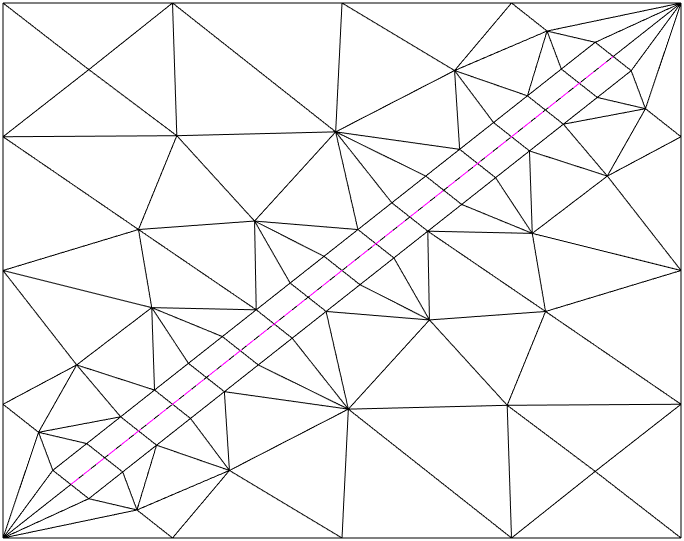
\includegraphics[width=\textwidth]{report/Images/Combining software/Wells as transfinite grids/cell_constraint_as_transfinite_delaunay_1.png}
        \end{subfigure}
        \begin{subfigure}[b]{0.35\textwidth}
            \centering
            \includegraphics[width=\textwidth]{report/Images/Combining software/Wells as transfinite grids/cell_constraint_as_transfinite_pebi_1.png}
        \end{subfigure}
        \caption{Well represented by 3-width transfinite grid.}
        \label{fig:trans-well-1}
    \end{subfigure}
    \begin{subfigure}[b]{\textwidth}
        \centering
        \begin{subfigure}[b]{0.35\textwidth}
            \centering
            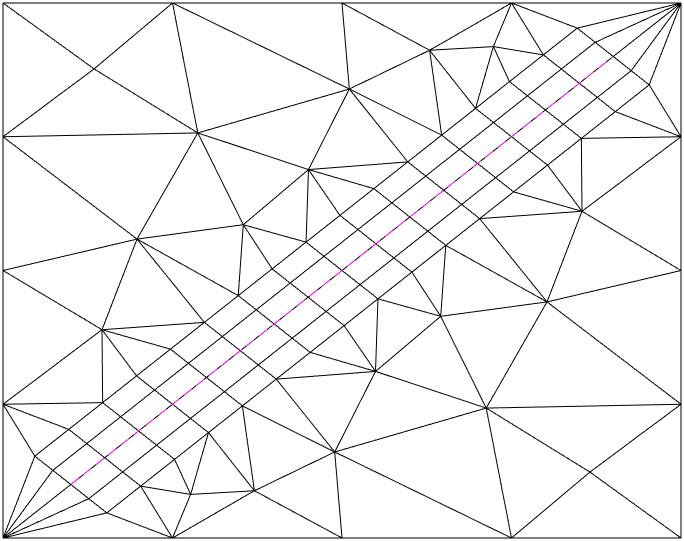
\includegraphics[width=\textwidth]{report/Images/Combining software/Wells as transfinite grids/cell_constraint_as_transfinite_delaunay_2.png}
        \end{subfigure}
        \begin{subfigure}[b]{0.35\textwidth}
            \centering
            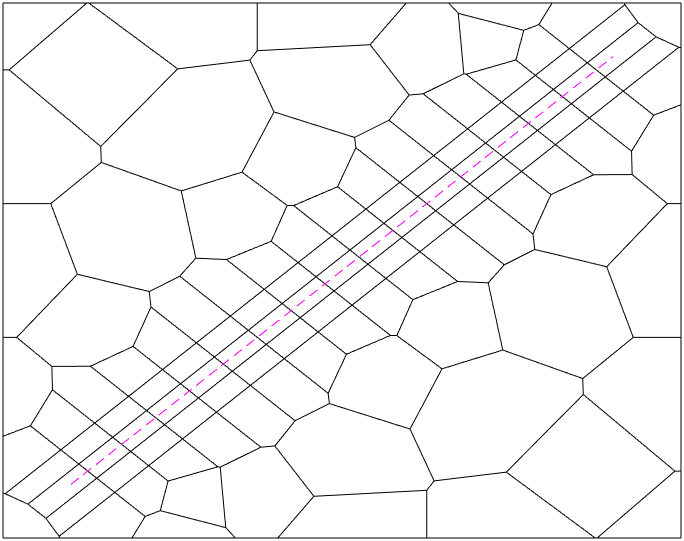
\includegraphics[width=\textwidth]{report/Images/Combining software/Wells as transfinite grids/cell_constraint_as_transfinite_pebi_2.png}
        \end{subfigure}
        \caption{Well represented by 5-width transfinite grid.}
        \label{fig:trans-well-2}
    \end{subfigure}
    \caption[Wells represented as transfinite grids.]{Wells represented as transfinite grids. The magenta line represents a well. The plots to the left are Delaunay grids before conversion, and the plots to the right are the resulting PEBI grids after conversion.}
    \label{fig:trans-wells}
\end{figure}


\paragraph{Faults and wells in MATLAB:}
Fault and well creation in \verb|pebiGrid2DGmsh| is done in MATLAB, and follows the same process as \verb|pebiGrid2D| from \textcite{UPR_thesis}. In short, this process places well sites and fault sites where they should be, and then later remove conflicting sites from the background grid. This means the Gmsh grid is constructed without having to worry about constraints, and then cleaned up later. An illustration of this process is shown in \autoref{fig:MATLAB-constraints}.

\begin{figure}[htp]
    \centering
    \begin{subfigure}[b]{0.32\textwidth}
        \centering
        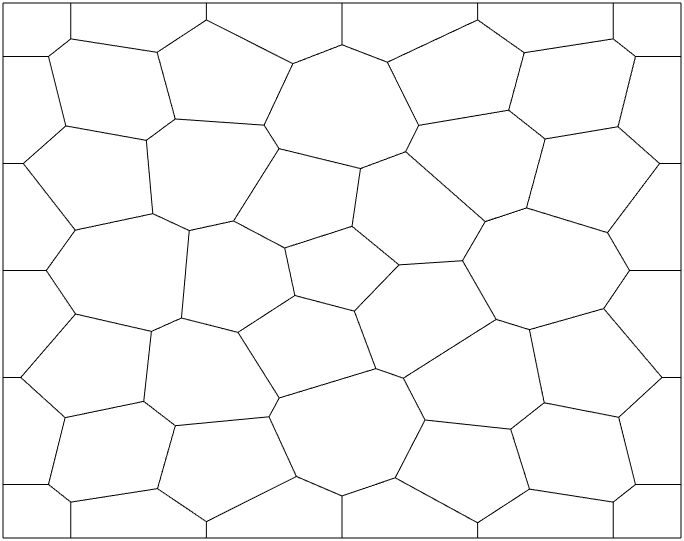
\includegraphics[width=\textwidth]{report/Images/Combining software/Constraints in MATLAB/constraints_MATLAB_1.png}
        \caption{Background grid.}
        \label{fig:MATLAB-constraints-1}
    \end{subfigure}
    \begin{subfigure}[b]{0.32\textwidth}
        \centering
        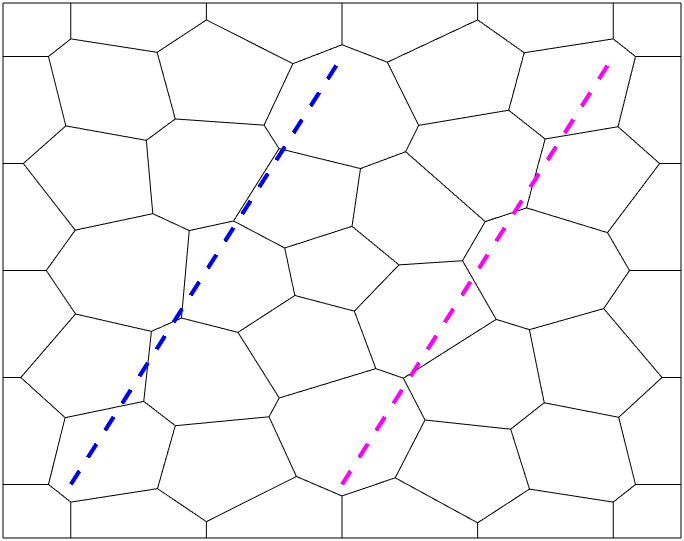
\includegraphics[width=\textwidth]{report/Images/Combining software/Constraints in MATLAB/constraints_MATLAB_2.png}
        \caption{Add constraints.}
        \label{fig:MATLAB-constraints-2}
    \end{subfigure}
    \begin{subfigure}[b]{0.32\textwidth}
        \centering
        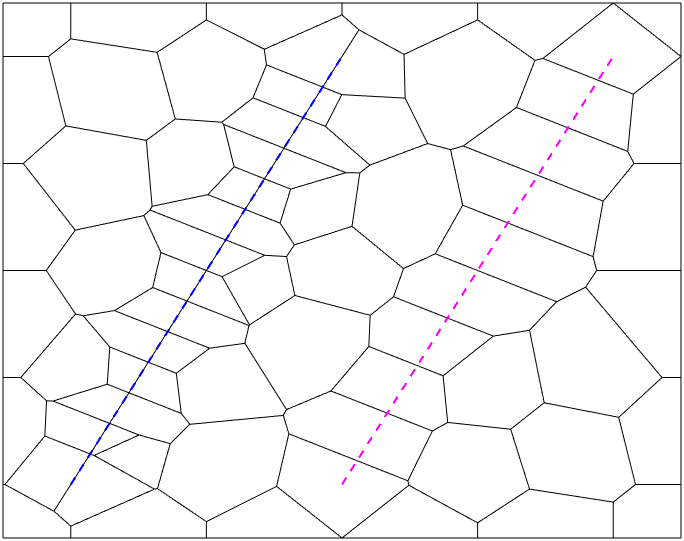
\includegraphics[width=\textwidth]{report/Images/Combining software/Constraints in MATLAB/constraints_MATLAB_3.png}
        \caption{Remove conflict points.}
        \label{fig:MATLAB-constraints-3}
    \end{subfigure}
    \caption[Creating faults and wells in MATLAB]{Creating faults and wells in MATLAB. The mesh in (\subref{fig:MATLAB-constraints-1}) is created using Gmsh. The constraints in (\subref{fig:MATLAB-constraints-2}) follow a familiar pattern -- the blue line is a fault, and the magenta line is a well. In (\subref{fig:MATLAB-constraints-3}), we have removed the conflict points and are left with a conforming grid.}
    \label{fig:MATLAB-constraints}
\end{figure}

\paragraph{Mesh refinement:}
The mesh refinement in \verb|gmsh4mrst| is done by using mesh size fields, as introduced in \autoref{sec:gmsh-modules}. Faults are used as inputs for one distance field, and wells are used as inputs for another. These fields are then used as input in their own threshold fields, and the minimum of these threshold fields are used as the final mesh size field. The distance constraints and the minimum size of the threshold fields are controlled by user-settable parameters, as discussed in Appendix~\ref{app:gmsh4mrst-arguments}. The maximum size of the threshold fields is set to the default cell size. An illustration of this process is shown in \autoref{fig:mesh-refinement}.

\begin{figure}[ht]
    \centering
    \begin{subfigure}[b]{0.32\textwidth}
        \centering
        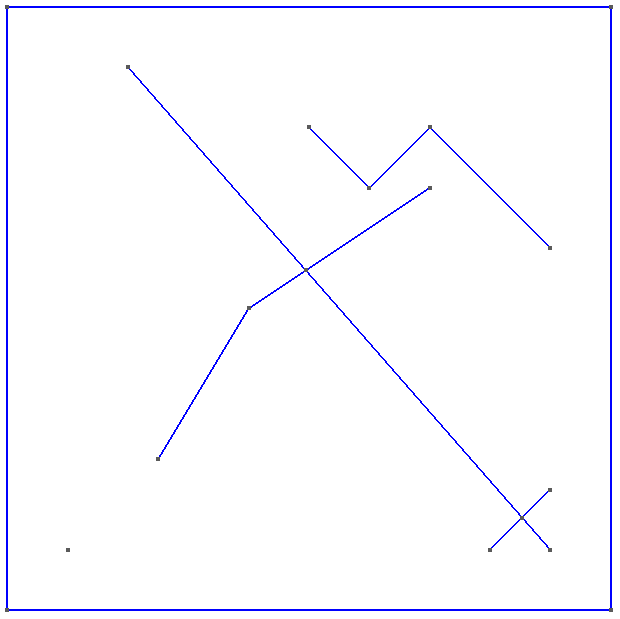
\includegraphics[width=\textwidth]{report/Images/Combining software/Mesh refinement/mesh_refinement_constraints.png}
        \caption{Constraints.}
        \label{fig:fig:mesh-refinement-constraints}
    \end{subfigure}
    \begin{subfigure}[b]{0.32\textwidth}
        \centering
        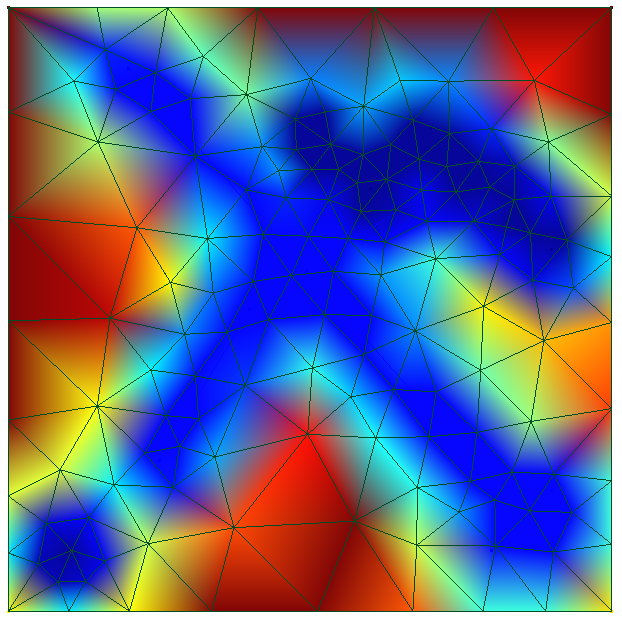
\includegraphics[width=\textwidth]{report/Images/Combining software/Mesh refinement/mesh_refinement_field.png}
        \caption{The mesh size field.}
        \label{fig:fig:mesh-refinement-field}
    \end{subfigure}
    \begin{subfigure}[b]{0.32\textwidth}
        \centering
        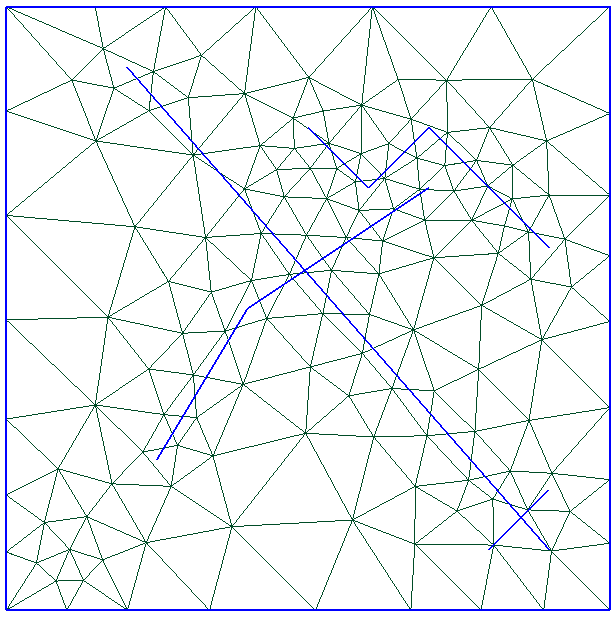
\includegraphics[width=\textwidth]{report/Images/Combining software/Mesh refinement/mesh_refinement_mesh.png}
        \caption{The produced mesh.}
        \label{fig:fig:mesh-refinement-mesh}
    \end{subfigure}
    \caption[Mesh refinement in \texttt{gmsh4mrst}.]{Mesh refinement in \texttt{gmsh4mrst}. The input of the mesh refinement is shown as constraints in (\subref{fig:fig:mesh-refinement-constraints}). Based on this, \texttt{gmsh4mrst} creates the mesh size field shown in (\subref{fig:fig:mesh-refinement-field}). The result is shown in (\subref{fig:fig:mesh-refinement-mesh}) as a Delaunay triangulation, but the method still applies when the triangulation is later converted to PEBI.}
    \label{fig:mesh-refinement}
\end{figure}


\paragraph{Combining MATLAB and Python:}
While MATLAB has a decent interface for calling Python methods, it is strict on the data conversion, and does not work when trying to send multi-dimensional- or cell arrays to Python. In order to bypass this, both the shape and constraints are converted to structs before being sent to Python, with constraints being converted to a multi-level struct. The result is that Python receives a MATLAB struct, which it reads as a Python dictionary, with an \verb|x|- and \verb|y|-key for each constraint. These keys point to a one-dimensional array, holding the x- and y-components of each constraint, respectively.

\subsubsection{Limitations of \texttt{gmsh4mrst}}
As \verb|gmsh4mrst| uses Gmsh to produce its meshes, the primary limitation of Gmsh -- that it produces Delaunay triangulations rather than PEBI grids -- creates limitations for \verb|gmsh4mrst| as well. While this has been worked around in \verb|pebiGrid2DGmsh|, it increases the work needed to produce good PEBI grids from Gmsh, and is the reason why we cannot encode faults and wells directly in the Gmsh mesh.

One key limitation of \verb|delaunayGrid2D| and \verb|pebiGrid2DGmshBase| arise from their use of transfinite grids. These grids cannot intersect, limiting the usability of the two methods -- \verb|delaunayGrid2D| will not work for cases where wells cross either other wells or faults, and \verb|pebiGrid2DGmshBase| will not work for cases where any constraints cross each other. While the methods work well when this is not the case, this places strict limitations on the usability of the methods.

Another thing worth mentioning is the structuredness of the transfinite grids produced in the above-mentioned methods. Due to the nature of transfinite grids, they produce highly structured subgrids. This is beneficial because it gives greater control of the produced grid, and thus great control of how it is converted into a PEBI grid, but may also be suboptimal if the grid is to be used for simulations or other work. In cases where this may be an issue, it would be better to use \verb|pebiGrid2DGmsh|, or any of the methods of the UPR module of MRST.

One key design goal of \verb|gmsh4mrst| was to create a drop-in replacement of Distmesh in \verb|pebiGrid2D|. While this is somewhat complete in \verb|pebiGrid2D|, it does not have complete API compitability, with many more arguments, as well as some that are not included in \verb|pebiGrid2DGmsh|. Some work is therefore needed if complete API compitability is wanted.

The final limitation worth mentioning is a distinct lack of feedback to the user, especially if something crashes. While basic argument parsing is done, any other errors are unhandled, creating confusing error messages. This is doubly true if anything goes wrong on the Python-side of things, where I have experienced everything from the connection between MATLAB and Python abruptly closing, to MATLAB crashing without any error message. This makes it hard for the user to understand what has gone wrong, and makes the program less robust.

One annoyance, although not directly a limit on how \verb|gmsh4mrst| can be used, is the following error message, being printed every time the MATLAB module of \verb|gmsh4mrst| is run. The error message comes from the use of \verb|gmshToMrst| for reading the file, and is present when using the latter method directly on a Gmsh mesh as well. As such, it is not a direct effect of \verb|gmsh4mrst|.
\begin{codeError}
Warning: No field 'faces.neighbors' found. Adding plausible values... proceed with caution! 
\end{codeError}

\subsubsection{Examples of \texttt{gmsh4mrst}}
% Funky domain
% Crossing constraints
% One more, c'mon